\documentclass[tikz,border=10pt]{standalone}
\usetikzlibrary{positioning, arrows.meta, calc, babel}
\usepackage[utf8]{inputenc}
\usepackage[T1]{fontenc}
\usepackage{lmodern}
\usepackage[english]{babel}
\usepackage{amsmath, amssymb, bm}

\begin{document}
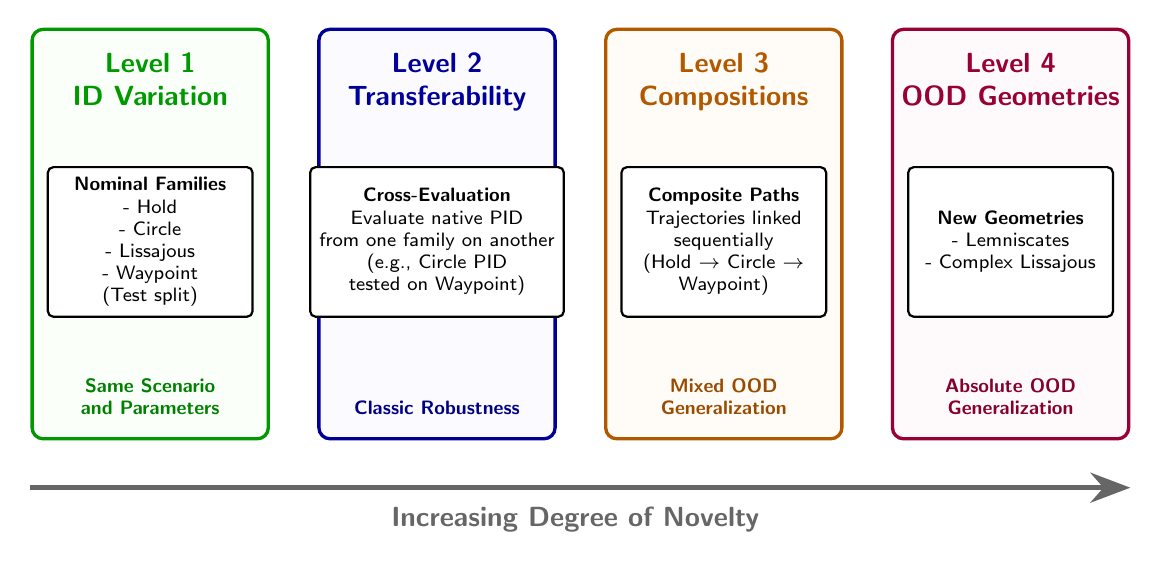
\begin{tikzpicture}[
  node distance=0.8cm and 0.5cm,
  align=center,
  font=\sffamily\small,
  % Estilos de columnas de fondo
  colbox/.style={draw, rectangle, rounded corners=4pt, minimum width=3.0cm, minimum height=5.2cm, line width=1.2pt},
  lvlbox/.style={draw, rectangle, rounded corners=2pt, minimum width=2.6cm, minimum height=1.9cm, fill=white, thick, font=\sffamily\scriptsize},
  % Estilos de flechas
  line/.style={draw, -{Stealth[scale=1.2]}, thick}
]

  % ==========================================
  % 4 COLUMNS OF EVALUATION LEVELS
  % ==========================================

  % --- COLUMN 1: LEVEL 1 (ID) ---
  \node[colbox, draw=green!60!black, fill=green!2] (col1) at (0,0) {};
  \node[anchor=north, font=\sffamily\bfseries, color=green!60!black, yshift=-0.2cm] (t1) at (col1.north) {Level 1\\ID Variation};
  \node[lvlbox] (lvl1) at ($(col1.center) + (0,-0.1)$) {
    \textbf{Nominal Families}\\
    - Hold\\
    - Circle\\
    - Lissajous\\
    - Waypoint\\
    (Test split)
  };
  \node[anchor=south, font=\sffamily\bfseries\scriptsize, color=green!50!black, yshift=0.2cm] at (col1.south) {Same Scenario\\and Parameters};

  % --- COLUMN 2: LEVEL 2 (Transferability) ---
  \node[colbox, draw=blue!60!black, fill=blue!2, right=0.6cm of col1] (col2) {};
  \node[anchor=north, font=\sffamily\bfseries, color=blue!60!black, yshift=-0.2cm] (t2) at (col2.north) {Level 2\\Transferability};
  \node[lvlbox] (lvl2) at ($(col2.center) + (0,-0.1)$) {
    \textbf{Cross-Evaluation}\\
    Evaluate native PID\\
    from one family on another\\
    (e.g., Circle PID\\
    tested on Waypoint)
  };
  \node[anchor=south, font=\sffamily\bfseries\scriptsize, color=blue!50!black, yshift=0.2cm] at (col2.south) {Classic Robustness};

  % --- COLUMN 3: LEVEL 3 (Mixed OOD) ---
  \node[colbox, draw=orange!70!black, fill=orange!3, right=0.6cm of col2] (col3) {};
  \node[anchor=north, font=\sffamily\bfseries, color=orange!70!black, yshift=-0.2cm] (t3) at (col3.north) {Level 3\\Compositions};
  \node[lvlbox] (lvl3) at ($(col3.center) + (0,-0.1)$) {
    \textbf{Composite Paths}\\
    Trajectories linked\\
    sequentially\\
    (Hold $\to$ Circle $\to$\\
    Waypoint)
  };
  \node[anchor=south, font=\sffamily\bfseries\scriptsize, color=orange!60!black, yshift=0.2cm] at (col3.south) {Mixed OOD\\Generalization};

  % --- COLUMN 4: LEVEL 4 (Absolute OOD) ---
  \node[colbox, draw=purple!80!black, fill=purple!2, right=0.6cm of col3] (col4) {};
  \node[anchor=north, font=\sffamily\bfseries, color=purple!80!black, yshift=-0.2cm] (t4) at (col4.north) {Level 4\\OOD Geometries};
  \node[lvlbox] (lvl4) at ($(col4.center) + (0,-0.1)$) {
    \textbf{New Geometries}\\
    - Lemniscates\\
    - Complex Lissajous
  };
  \node[anchor=south, font=\sffamily\bfseries\scriptsize, color=purple!70!black, yshift=0.2cm] at (col4.south) {Absolute OOD\\Generalization};

  % ==========================================
  % BOTTOM ARROW SHOWING INCREASING DIFFICULTY
  % ==========================================
  \draw[line, line width=2.0pt, color=black!60] 
    ($(col1.south west) + (0, -0.6)$) -- node[below, font=\sffamily\bfseries\color{black!70}, yshift=-0.1cm] {Increasing Degree of Novelty} ($(col4.south east) + (0, -0.6)$);

\end{tikzpicture}
\end{document}
